\lstinputlisting[language=bash,basicstyle=\small]{python_codes/fieldstone_11/keywords}

The setup is identical to the one of the Stone \ref{f10}.

The difference lies in how we solve the Stokes equation. This stone does not rely on 
the penalty method (Section \ref{sec:penalty}) 
but instead used a mixed formulation, i.e. we solve for both 
velocity and pressure at the same time (see Section~\ref{sec:mixed}).

In the case when free slip boundary conditions are applied on all 
6 faces of the cube we know that there is a pressure nullspace, i.e.
that the pressure can be computed up to a constant. In order to 
remove this nullspace one must add an additional constraint 
We here choose to (somewhat arbitrarily) enforce that the average pressure 
over the whole domain is zero:
\[
<p>=\frac{1}{|\Omega|} \int_\Omega p dV =0 
\]
Since the code relies of discontinuous zero-th order polynomial shape functions 
for pressure this condition simply writes (and since $|\Omega|=1$):
\[
<p>=\frac{1}{|\Omega|} \int_\Omega p dV =  \sum_{e} \int_{\Omega_e} p dV = \sum_e p_e V_e = h^3 \sum_e p_e =0
\]
Dividing all by $h^3$, the condition becomes simply:
\[
p_1 + p_2 + p_3 + ... + p_{nel} = 0
\]
How this constraint is incorporated in the Stokes matrix is explained in Section~\ref{ss_pnorm}.

It is also important to remember that if one now switches to a free surface at the top then 
the null space is absent from the equations and the constraint should be removed/switched off.

The pressure normalisation is controled by the boolean {\sl pnormalise} in the code. 
Since the pressure constraint adds a line to the global FE, we then logically have:
\begin{lstlisting}
if pnormalise:
   a_mat = np.zeros((Nfem+1,Nfem+1),dtype=np.float64) 
   rhs   = np.zeros(Nfem+1,dtype=np.float64)    
else:
   a_mat = np.zeros((Nfem,Nfem),dtype=np.float64)
   rhs   = np.zeros(Nfem,dtype=np.float64)       
\end{lstlisting} 
Once the solve has been done, we retrieve the separate velocity and pressure fields as follows:
\begin{lstlisting}
u,v,w=np.reshape(sol[0:NfemV],(nnp,3)).T
p=sol[NfemV:Nfem]
\end{lstlisting} 
and the Lagrange multiplier is a scalar at the bottom of the array:
\begin{lstlisting}
if pnormalise:
   print("     -> Lagrange multiplier: %.4es" % sol[Nfem])
\end{lstlisting} 

It is quite easy in python to visualise the matrix structure 
with the spy function:
\begin{lstlisting}
plt.spy(a_mat)
\end{lstlisting} 
and we see that we indeed recover
the block structure with a zero block for the pressure-pressure entries.  
\begin{center}
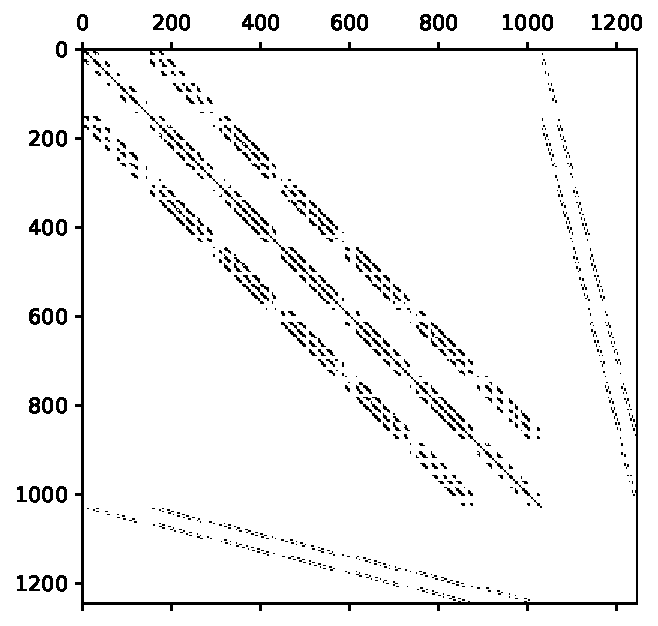
\includegraphics[width=7cm]{python_codes/fieldstone_11/results/matrix6x6x6.pdf}
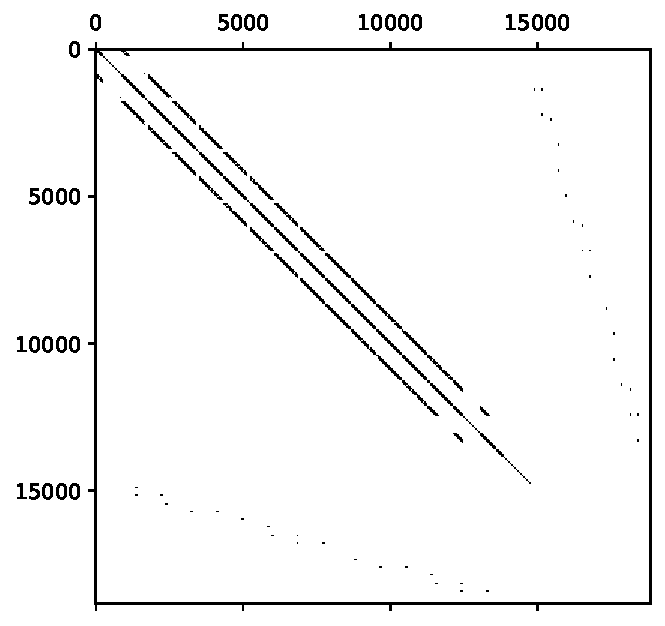
\includegraphics[width=7cm]{python_codes/fieldstone_11/results/matrix16x16x16.pdf}\\
{\captionfont Sparsity pattern of the Stokes matrix for a 6x6x6 mesh (left) and a 16x16x16 mesh (right).}
\end{center}

\begin{center}
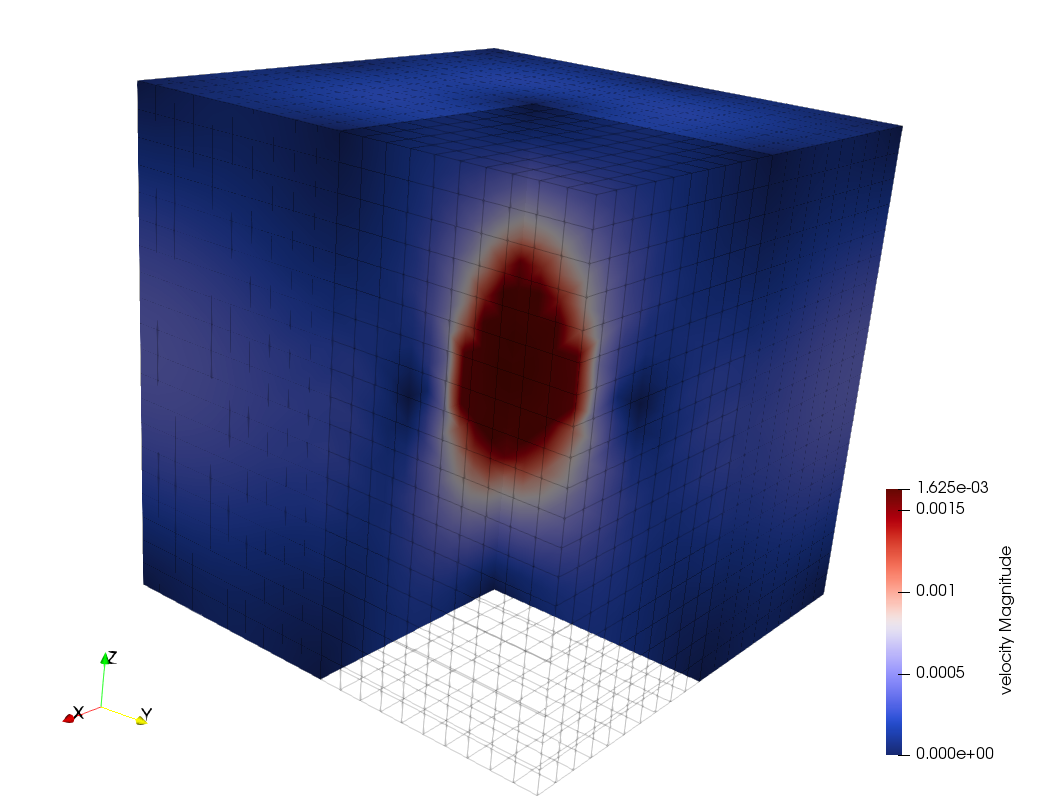
\includegraphics[width=7cm]{python_codes/fieldstone_11/results/vel}
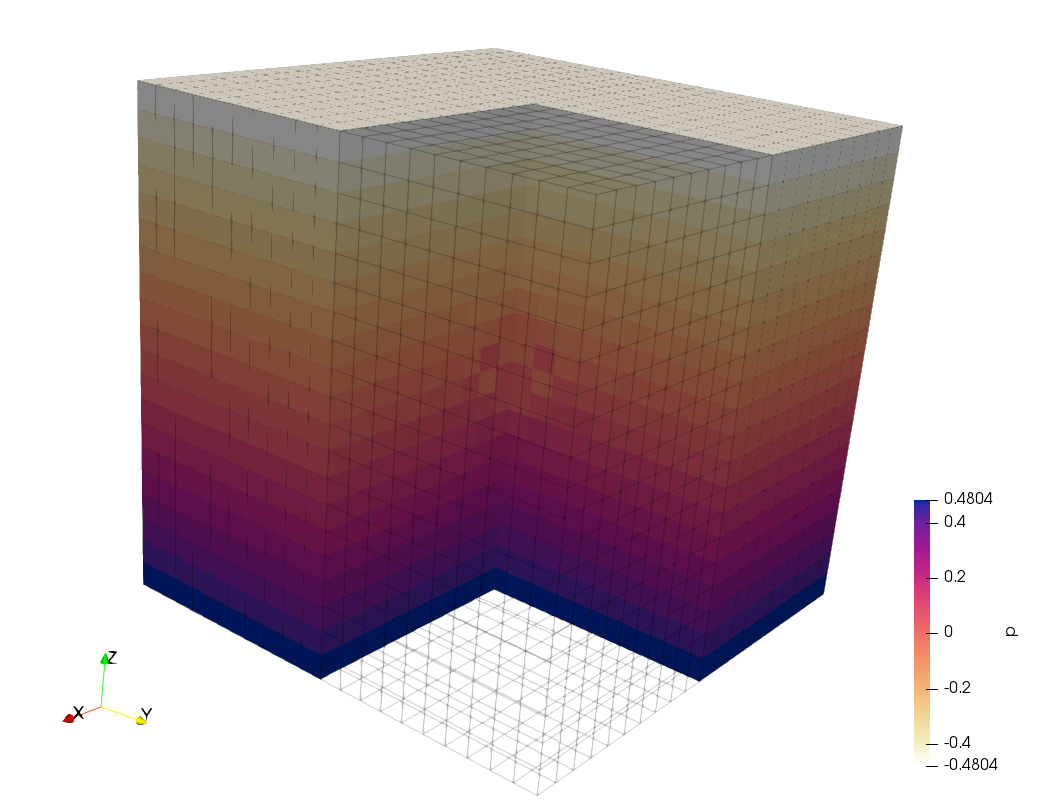
\includegraphics[width=7cm]{python_codes/fieldstone_11/results/press}
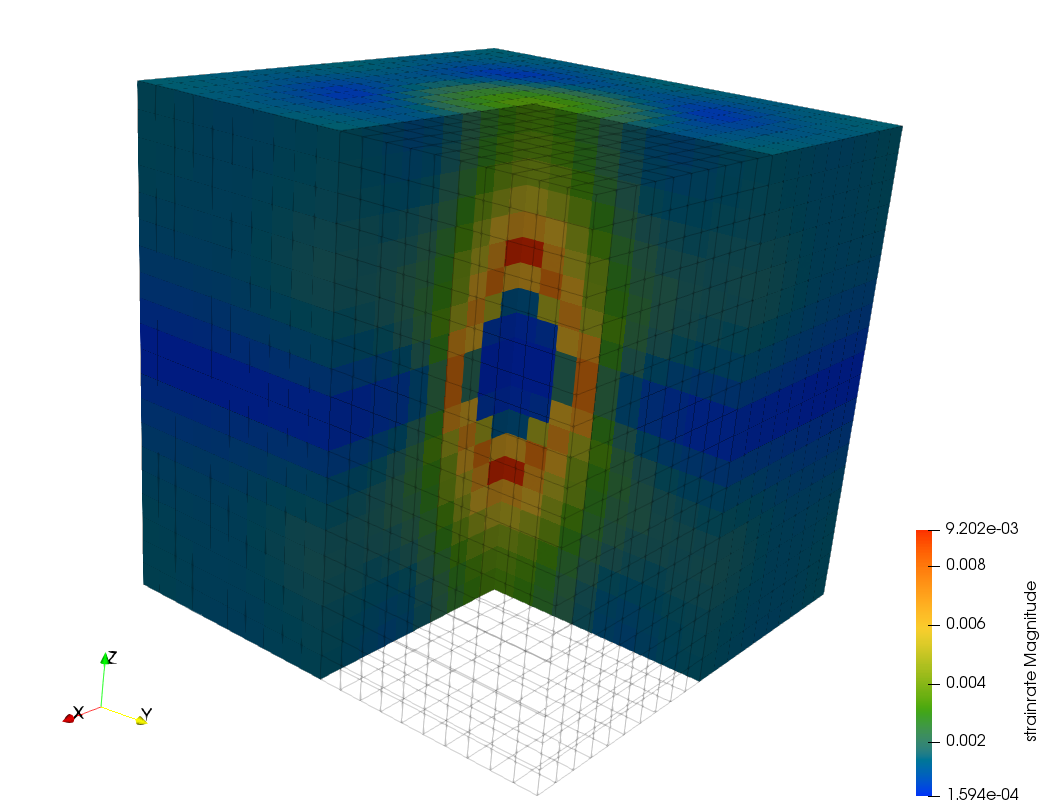
\includegraphics[width=8cm]{python_codes/fieldstone_11/results/sr}\\
{\captionfont Velocity, pressure and effective strain rate fields for a 20x20x20 mesh.}
\end{center}
